\chapter{Technologies used}
\label{chapter:technologiesUsed}


\section{The Spring Framework}
\label{section:springBootFramework}

\subsection{Spring Boot}
\label{subsection:springBoot}

\subsection{Spring Security}
\label{subsection:proposedSolution}

\subsection{Spring JDBC}
\label{subsection:springJDBC}


\section{ReactJS Framework}
\label{section:reactJSFramework}

\section{Redux}
\label{section:redux}


\section{MySQL Database}
\label{section:mysqlDatabase}

% Item example: 

% \begin{itemize}
% 	\item content of item1
%  	\item content of item2
%  	\item content of item3
% \end{itemize}

% Figure example 

% $\ldots$ (see Figure \ref{swarmsize})

% \begin{figure}[htbp]
% 	\centerline{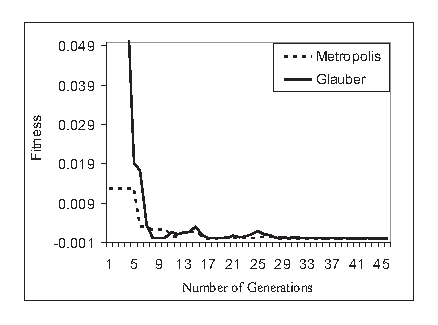
\includegraphics{Fig/FitEvol.eps}}  
% 	\caption{The evolution of the swarm size during the GA generations. This results were obtained for the $f_2$ test function with 5 dimensions.}
% 	\label{swarmsize}
% \end{figure}


% Table example: (see Table \ref{tab3PSO})


% \begin{table}[htbp]
% 	\caption{The parameters of the PSO algorithm (the micro level algorithm) used to compute the fitness of a GA chromosome.}
% 	\label{tab3PSO}
% 		\begin{center}
% 			\begin{tabular}{p{220pt}c}

% 				\textbf{Parameter}& \textbf{Value} \\
% 				\hline\hline
%  				Number of generations& 50 \\
%  				Number of function evaluations/generation& 10 \\
%  				Number of dimensions of the function to be optimized& 5 \\
%  				Learning factor $c_{1}$& 2 \\
%  				Learning factor $c_{2}$ & 1.8\\
%  				Inertia weight& 0.5 + $\frac{rand()}{2}$\\
		
% 			\end{tabular}
% 		\end{center}
% \end{table}


